% Apendice - LaTeX

% ----------------------------------------------------------
\chapter{LaTeX}\label{ap:latex}
% ----------------------------------------------------------

Para o desenvolvimento dessa monografia utilizou-se uma ferramenta denominada TeX, um processador de texto baseado em comandos e macros. Normalmente é grafado usando a macro \texttt{\detokenize{\TeX}}, resultando em \TeX. 

Não é comum o uso do \TeX\ por si só. Utiliza-se uma outra ferramenta denominada LaTeX (grafada \LaTeX), uma série de macros definidas para auxiliar o desenvolvimento.

Essa abordagem é muito utilizada no meio acadêmico e científico, pois o ponto mais importante dessa ferramenta é o conteúdo. O design final ficará sempre para o compilador gerar. Isso evita erros de formatação, como por exemplo devido a diferenças entre versões de programas.

Congressos e revistas científicas já disponibilizam arquivos no formato \texttt{.sty}\footnote{Modelo de estilos \TeX.} para que os pesquisadores enviem os artigos preenchidos em \texttt{.pdf} formatado conforme modelo próprio. Dessa forma todos os artigos seguirão o mesmo formato, auxiliando também os pesquisadores a escreverem os documentos rapidamente.

Por ser um documento de texto no formato \texttt{.tex}, qualquer editor comum como o Bloco de Notas do Windows pode ser utilizado. Dessa forma a compilação é feita por meio da linha de comando, com algumas opções de compiladores. As mais utilizadas são \texttt{pdflatex} e \texttt{xelatex}.

O meio mais utilizado para escrita de documentos \LaTeX\ de forma a facilitar a compilação são programas próprios. Existem diversas opções, mas as mais utilizadas são MiKTeX\footnote{\url{http://miktex.org/}} para Windows e MacTeX\footnote{\url{http://tug.org/mactex}} para Mac OS X. O programa utilizado para esse documento foi o TeXworks, um editor de texto para \TeX\ multiplataforma e de código aberto, conforme imagem \ref{fig:texworks}.

\begin{figure}[htb]
	\caption{\label{fig:texworks}TeXworks, programa utilizado para escrever o código \TeX}
	\begin{center}
		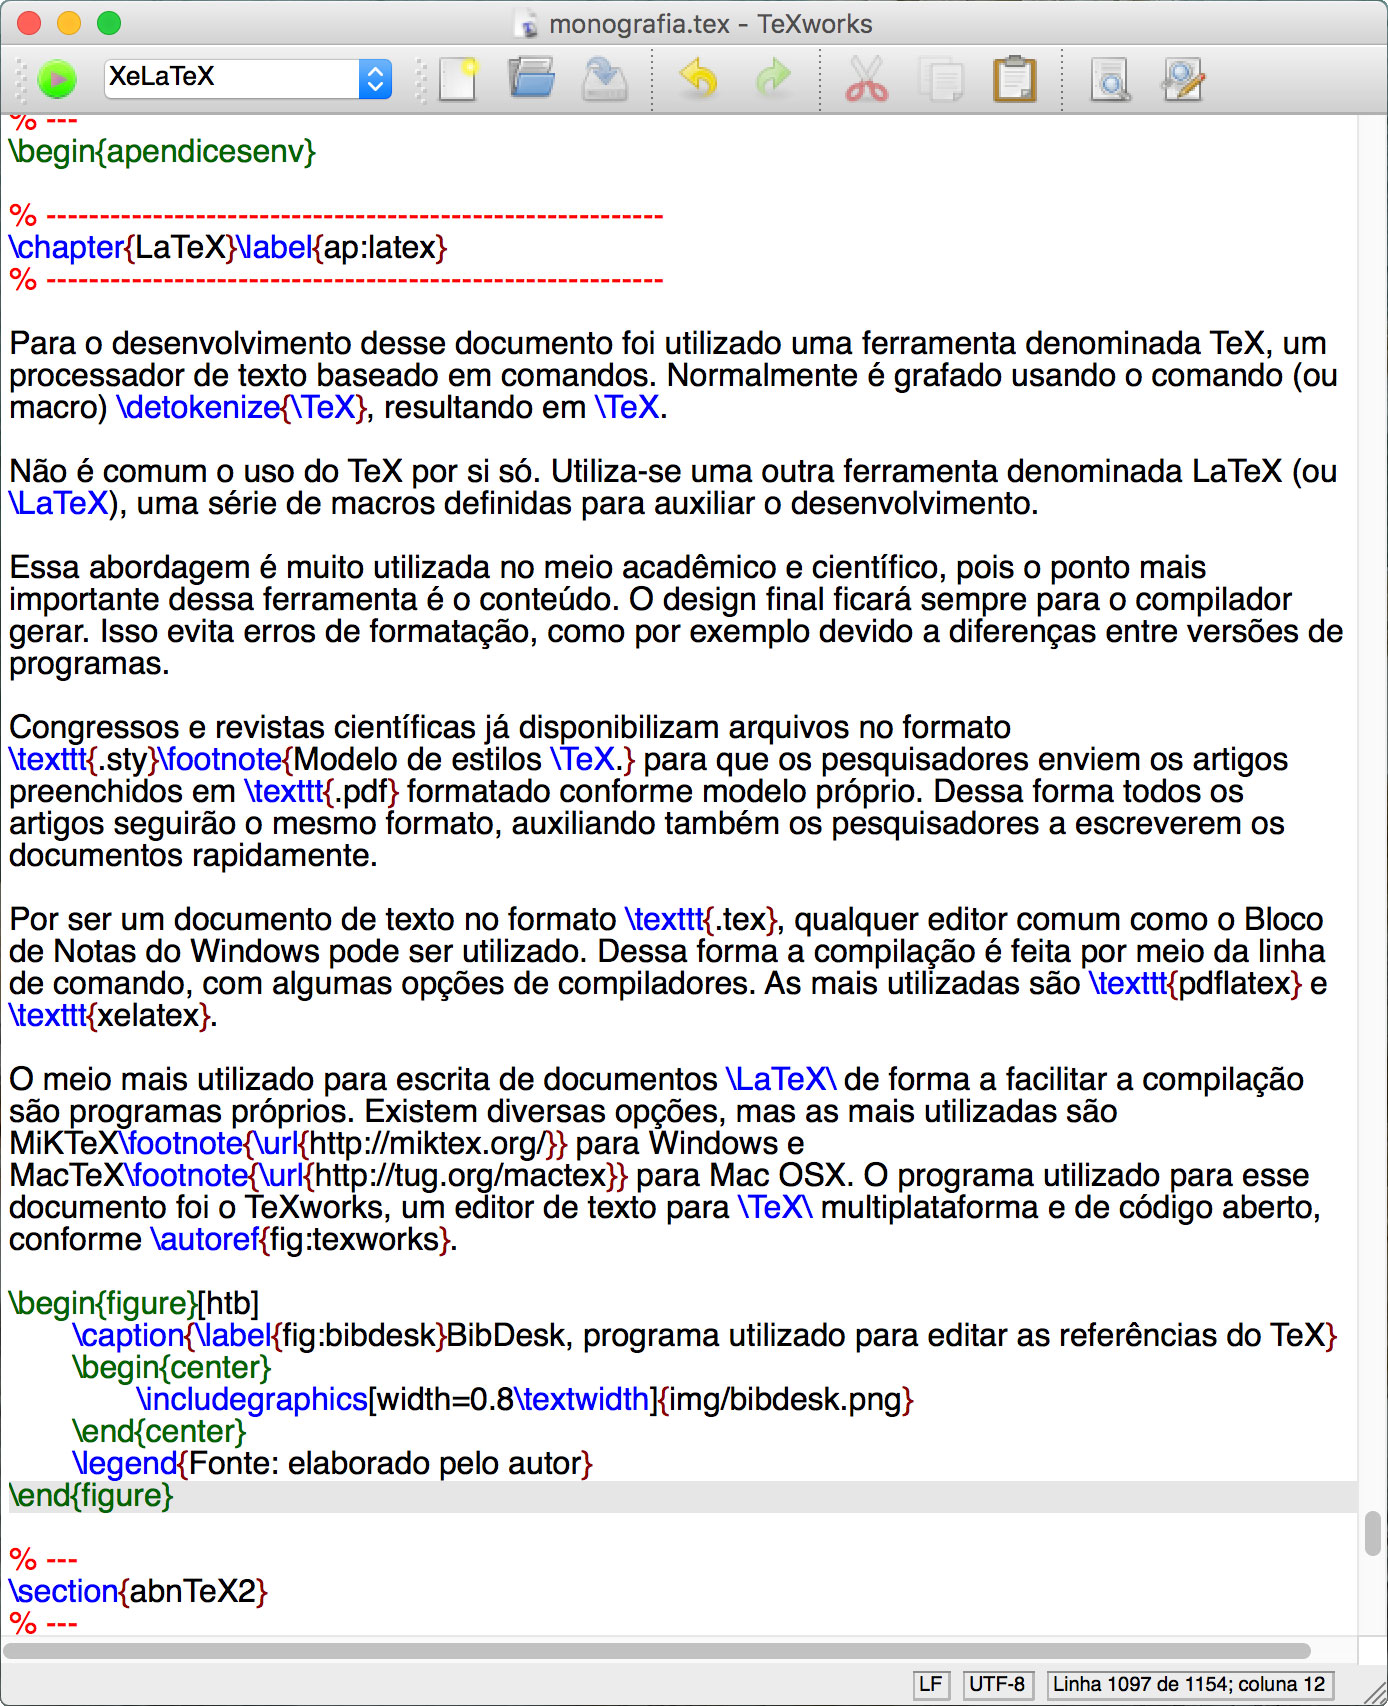
\includegraphics[width=0.65\textwidth]{img/texworks.jpg}
	\end{center}
	\legend{Fonte: elaborado pelo autor}
\end{figure}

% ---
\section{abnTeX2}
% ---

Devido a esse Trabalho de Conclusão de Curso seguir as normas ABNT\footnote{Associação Brasileira de Normas Técnicas.} para escrita e formatação de documentos científicos, utilizou-se a biblioteca de macros abnTeX2 (\abnTeX)\footnote{\url{https://github.com/abntex/abntex2}} para formatação do documento conforme as normas vigentes. Essa biblioteca é livre, com código fonte aberto e disponível para qualquer um auxiliar.

Uma ferramenta muito útil disponível com o \abnTeX\ é a criação das Referências Bibliográficas no formato ABNT de forma automática. Para tal, é criado um arquivo \texttt{.bib} com todas as informações de citações e referências utilizadas no texto.

As chaves de citação são os valores que serão utilizados nas macros do \abnTeX\ para que as referências sejam corretamente configuradas. Por exemplo, se desejamos referenciar um artigo de \citeonline{windows10-iot}, adicionamos todas as informações como nome dos autores, organização, data, edição, entre outros, e adicionamos a chave \texttt{windows10-iot}. 

Utilizando a macro \texttt{\detokenize{\cite{windows10-iot}}}, no local ficará o texto \cite{windows10-iot}, e nas referências será adicionado conforme modelo ABNT: \texttt{MICROSOFT. A Internet das suas coisas. https://dev.windows.com/pt-br/iot, 2015.} Para citações \textit{inline}, ou na mesma linha, o comando \texttt{\detokenize{\citeonline{windows10-iot}}} é utilizado, gerando o texto \citeonline{windows10-iot}.

O arquivo \texttt{.bib} pode ser criado manualmente ou por meio de programas. Para esse artigo foi utilizado o programa BibDesk\footnote{\url{http://bibdesk.sourceforge.net/}} para Mac OSX, conforme \autoref{fig:bibdesk}. Esse programa já cria o arquivo no formato correto com as chaves de citação configuradas.

\begin{figure}[htb]
	\caption{\label{fig:bibdesk}BibDesk, programa utilizado para editar as referências do \TeX}
	\begin{center}
		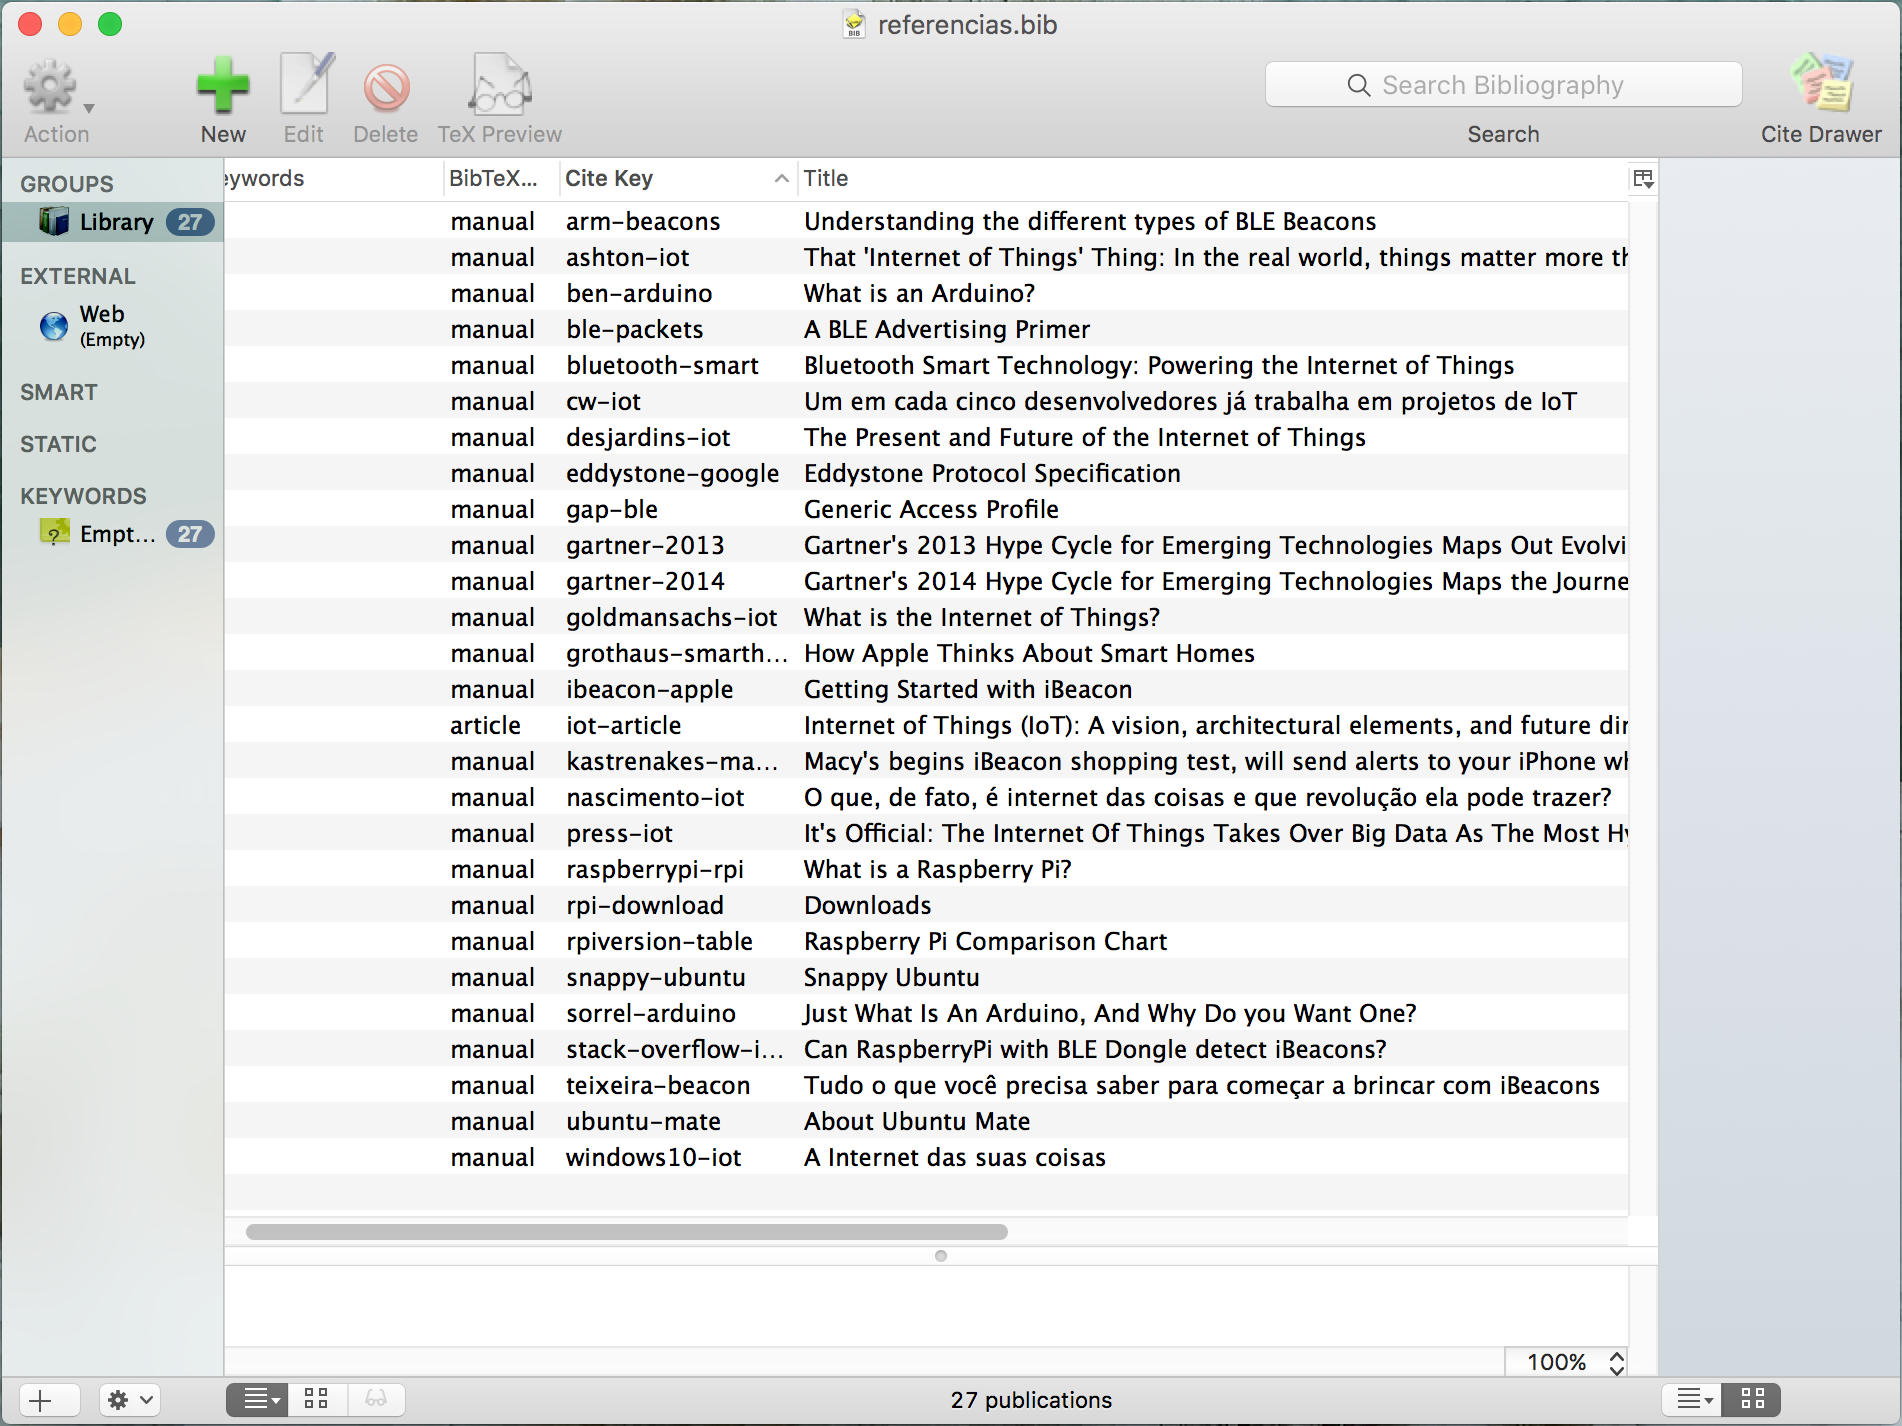
\includegraphics[width=0.8\textwidth]{img/bibdesk.png}
	\end{center}
	\legend{Fonte: elaborado pelo autor}
\end{figure}

Além de formatar o documento, \abnTeX\ também disponibiliza macros para criação de conteúdo citados na ABNT. Por exemplo, tabelas que seguem o formato do IBGE\footnote{Instituto Brasileiro de Geografia e Estatística} podem ser facilmente criadas com macros disponíveis, como exemplo da \autoref{table:ble-physical2}.

\begin{table}[htb]
     \IBGEtab{
          \caption{Exemplo de tabela gerada com o \LaTeX}
          \label{table:ble-physical2}
     }{
          \begin{tabular}{ccc}
               \toprule
                    & BLE & Classic \\
               \midrule \midrule
                    Modulação & GFSK 0.45 a 0.55 & GFSK 0.28 a 0.35 \\
               \midrule
                    Velocidade de Transferência & 1 Mbit/s & 1 Mbit/s \\
               \midrule 
                    Canais & 40 & 79 \\
               \midrule 
                    Espaçamento & 2 MHz & 1 MHz \\
               \bottomrule
          \end{tabular}
     }{
          \fonte{\cite{ble-packets}}
     }
\end{table}

O código para geração da \autoref{table:ble-physical2}, conforme a documentação da \abnTeX\, é:
\\ % para pular mais uma linha
\begin{verbatim}
\begin{table}[htb]
     \IBGEtab{
          \caption{\textit{BLE Physical Layer}}
          \label{table:ble-physical}
     }{
          \begin{tabular}{ccc}
               \toprule
                    & BLE & Classic \\
               \midrule \midrule
                    Modulação & GFSK 0.45 a 0.55 & GFSK 0.28 a 0.35 \\
               \midrule
                    Velocidade de Transferência & 1 Mbit/s & 1 Mbit/s \\
               \midrule 
                    Canais & 40 & 79 \\
               \midrule 
                    Espaçamento & 2 MHz & 1 MHz \\
               \bottomrule
          \end{tabular}
     }{
          \fonte{\cite{ble-packets}}
     }
\end{table}
\end{verbatim}

Diversas razões podem ser elencadas a favor do uso do \LaTeX\ e \abnTeX\ nessa monografia, entre elas:

\begin{alineas}
	\item Facilidade de criação do conteúdo: \abnTeX\ já formata o documento conforme as normas ABNT, necessitando somente colocar o conteúdo interno;
	\item Evitar erros de formatação ao alterar o conteúdo do arquivo: muito comum quando utilizado o Microsoft Word, ao alterar o conteúdo de uma seção, as partes subsequentes facilmente perdem a formatação, sendo necessário uma revisão minunciosa para que esses erros sejam evitados;
	\item Continuação dos outros relatórios: como o autor gostaria de aprender essa tecnologia, utilizou para desenvolver a proposta desse trabalho. Portanto, para facilitar, continuou os outros relatórios utilizando a mesma ferramenta;
\end{alineas}

O código dessa monografia, assim como a versão final em \texttt{.pdf} pode ser acessado pelo repositório no GitHub\footnote{\url{https://github.com/gabrielboliveira/Monografia-Peacon}}. Está disponível para livre consulta, tanto de professores quanto de alunos interessados em saber mais sobre o \LaTeX.